% In S^1, the loop gamma equals c - d, seen as the boundary of a 2-simplex.
% Source: book/tex/homology/singular.tex (§ An explicit boundary in S^1).
\documentclass[border=2mm]{standalone}
\usepackage{tikz}
\usetikzlibrary{arrows.meta}
\definecolor{heavygreen}{rgb}{0,0.5,0}
\begin{document}
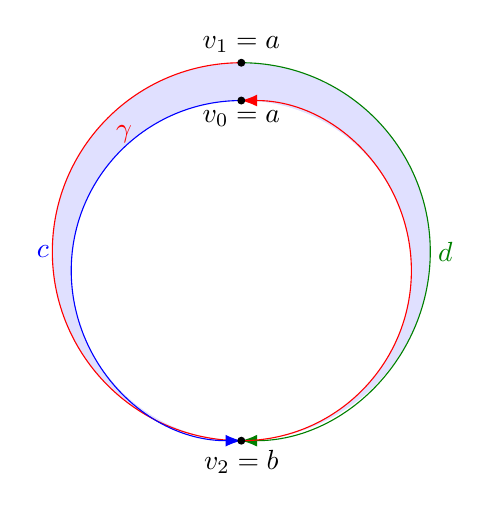
\begin{tikzpicture}[>={Latex[length=2mm]}, scale=2.4]
  % 2-simplex region: outer disk minus inner disk
  \fill[blue!12] (0,0) circle (1);
  \fill[white] (0,-0.1) circle (0.9);
  % outer circle: right half = d (green), left half = red
  \draw[heavygreen, ->] (0,1) arc (90:-90:1);
  \draw[red] (0,1) arc (90:270:1);
  % inner circle: left half = c (blue), right half = red (gamma)
  \draw[blue, ->] (0,0.8) arc (90:270:0.9);
  \draw[red, ->] (0,-1) arc (270:450:0.9);
  % vertices
  \fill (0,0.8) circle (0.6pt); \node[below] at (0,0.8) {$v_0 = a$};
  \fill (0,1) circle (0.6pt); \node[above] at (0,1) {$v_1 = a$};
  \fill (0,-1) circle (0.6pt); \node[below] at (0,-1) {$v_2 = b$};
  \node[red] at (-0.62,0.62) {$\gamma$};
  \node[blue] at (-1.05,0) {$c$};
  \node[heavygreen] at (1.08,0) {$d$};
\end{tikzpicture}
\end{document}
